% GEOMIRA export: TikZ. One unit is 30bp (40 px on screen).
% Needs \usepackage{tikz} and \usepackage{amssymb}.
% Warning: the color "notacolour" of x_a cannot be read: drawn in the default ink
% Warning: the label of t3 has a character TeX cannot write ("é", U+00E9): written as ?
% Warning: the label of t3 has a character TeX cannot write ("☃", U+2603): written as ?
% Warning: the label of t3* has a character TeX cannot write ("é", U+00E9): written as ?
% Warning: the label of t3* has a character TeX cannot write ("☃", U+2603): written as ?
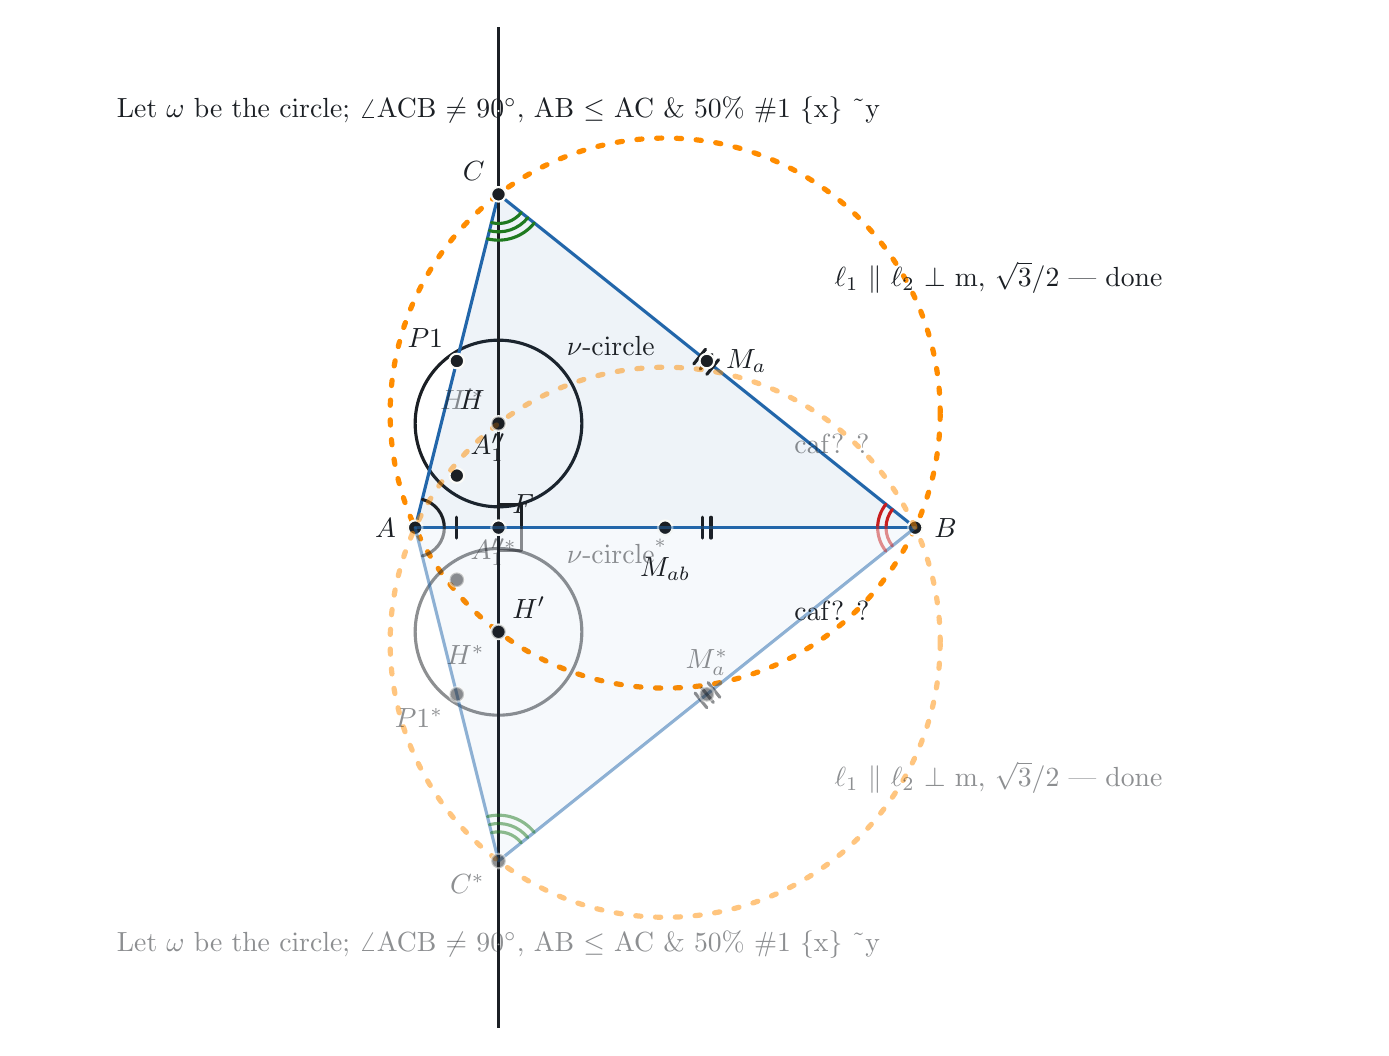
\begin{tikzpicture}[x=30bp, y=30bp, line cap=round, line join=round]
\definecolor{gmc0}{HTML}{1B1F24}
\definecolor{gmc1}{HTML}{2266AA}
\definecolor{gmc2}{HTML}{FF8C00}
\definecolor{gmc3}{HTML}{C81E1E}
\definecolor{gmc4}{HTML}{1F7A1F}
\definecolor{gmc5}{HTML}{FBFBF8}
\clip (-4.65,-6) rectangle (11.35,6);
% ν
\draw[gmc0, line width=1.125bp] (2,1.25) arc[start angle=0, end angle=360, radius=1];
% tri
\fill[gmc1, fill opacity=0.08] (0,0) -- (6,0) -- (1,4) -- cycle;
\draw[gmc1, line width=1.125bp] (0,0) -- (6,0);
\draw[gmc1, line width=1.125bp] (6,0) -- (1,4);
\draw[gmc1, line width=1.125bp] (1,4) -- (0,0);
% ω
\draw[gmc2, line width=1.875bp, dash pattern=on 1.875bp off 5.25bp] (6.3001,1.375) arc[start angle=0, end angle=360, radius=3.30009];
% x_a
\draw[gmc0, line width=1.125bp] (1,7.7) -- (1,-7.7);
% m1
\draw[gmc0, line width=1.125bp] (0.5,0.125) -- (0.5,-0.125);
% m2
\draw[gmc0, line width=1.125bp] (3.45,0.125) -- (3.45,-0.125);
\draw[gmc0, line width=1.125bp] (3.55,0.125) -- (3.55,-0.125);
% m3
\draw[gmc0, line width=1.125bp, dash pattern=on 6.75bp off 5.25bp] (3.5,1.8399) -- (3.6562,2.0351);
\draw[gmc0, line width=1.125bp, dash pattern=on 6.75bp off 5.25bp] (3.4219,1.9024) -- (3.5781,2.0976);
\draw[gmc0, line width=1.125bp, dash pattern=on 6.75bp off 5.25bp] (3.3438,1.9649) -- (3.5,2.1601);
% a1
\draw[gmc0, line width=1.125bp] (0.35,0) arc[start angle=0, end angle=75.9638, radius=0.35];
% a2
\draw[gmc3, line width=1.125bp] (5.7267,0.2186) arc[start angle=141.3402, end angle=180, radius=0.35];
\draw[gmc3, line width=1.125bp] (5.6486,0.2811) arc[start angle=141.3402, end angle=180, radius=0.45];
% a3
\draw[gmc4, line width=1.125bp] (0.9151,3.6605) arc[start angle=-104.0362, end angle=-38.6598, radius=0.35];
\draw[gmc4, line width=1.125bp] (0.8909,3.5634) arc[start angle=-104.0362, end angle=-38.6598, radius=0.45];
\draw[gmc4, line width=1.125bp] (0.8666,3.4664) arc[start angle=-104.0362, end angle=-38.6598, radius=0.55];
% r1
\draw[gmc0, line width=1.125bp] (1.275,0) -- (1.275,0.275) -- (1,0.275);
% A
\filldraw[fill=gmc0, draw=gmc5, line width=0.75bp] (0,0) circle[radius=2.625bp];
% B
\filldraw[fill=gmc0, draw=gmc5, line width=0.75bp] (6,0) circle[radius=2.625bp];
% C
\filldraw[fill=gmc0, draw=gmc5, line width=0.75bp] (1,4) circle[radius=2.625bp];
% H
\filldraw[fill=gmc0, draw=gmc5, line width=0.75bp] (1,1.25) circle[radius=2.625bp];
% F
\filldraw[fill=gmc0, draw=gmc5, line width=0.75bp] (1,0) circle[radius=2.625bp];
% M_a
\filldraw[fill=gmc0, draw=gmc5, line width=0.75bp] (3.5,2) circle[radius=2.625bp];
% M_{ab}
\filldraw[fill=gmc0, draw=gmc5, line width=0.75bp] (3,0) circle[radius=2.625bp];
% H'
\filldraw[fill=gmc0, draw=gmc5, line width=0.75bp] (1,-1.25) circle[radius=2.625bp];
% A_1''
\filldraw[fill=gmc0, draw=gmc5, line width=0.75bp] (0.5,0.625) circle[radius=2.625bp];
% P1
\filldraw[fill=gmc0, draw=gmc5, line width=0.75bp] (0.5,2) circle[radius=2.625bp];
% t1
\filldraw[fill=gmc0, draw=gmc5, line width=0.75bp] (1,5) circle[radius=0bp];
% t2
\filldraw[fill=gmc0, draw=gmc5, line width=0.75bp] (7,3) circle[radius=0bp];
% t3
\filldraw[fill=gmc0, draw=gmc5, line width=0.75bp] (5,-1) circle[radius=0bp];
% ν*
\draw[gmc0, line width=1.125bp, draw opacity=0.5] (2,-1.25) arc[start angle=0, end angle=360, radius=1];
% tri*
\fill[gmc1, fill opacity=0.04] (0,0) -- (6,0) -- (1,-4) -- cycle;
\draw[gmc1, line width=1.125bp, draw opacity=0.5] (0,0) -- (6,0);
\draw[gmc1, line width=1.125bp, draw opacity=0.5] (6,0) -- (1,-4);
\draw[gmc1, line width=1.125bp, draw opacity=0.5] (1,-4) -- (0,0);
% ω*
\draw[gmc2, line width=1.875bp, dash pattern=on 1.875bp off 5.25bp, draw opacity=0.5] (6.3001,-1.375) arc[start angle=0, end angle=360, radius=3.30009];
% m3*
\draw[gmc0, line width=1.125bp, dash pattern=on 6.75bp off 5.25bp, draw opacity=0.5] (3.6562,-2.0351) -- (3.5,-1.8399);
\draw[gmc0, line width=1.125bp, dash pattern=on 6.75bp off 5.25bp, draw opacity=0.5] (3.5781,-2.0976) -- (3.4219,-1.9024);
\draw[gmc0, line width=1.125bp, dash pattern=on 6.75bp off 5.25bp, draw opacity=0.5] (3.5,-2.1601) -- (3.3438,-1.9649);
% a1*
\draw[gmc0, line width=1.125bp, draw opacity=0.5] (0.0849,-0.3395) arc[start angle=-75.9638, end angle=0, radius=0.35];
% a2*
\draw[gmc3, line width=1.125bp, draw opacity=0.5] (5.65,0) arc[start angle=180, end angle=218.6598, radius=0.35];
\draw[gmc3, line width=1.125bp, draw opacity=0.5] (5.55,0) arc[start angle=180, end angle=218.6598, radius=0.45];
% a3*
\draw[gmc4, line width=1.125bp, draw opacity=0.5] (1.2733,-3.7814) arc[start angle=38.6598, end angle=104.0362, radius=0.35];
\draw[gmc4, line width=1.125bp, draw opacity=0.5] (1.3514,-3.7189) arc[start angle=38.6598, end angle=104.0362, radius=0.45];
\draw[gmc4, line width=1.125bp, draw opacity=0.5] (1.4295,-3.6564) arc[start angle=38.6598, end angle=104.0362, radius=0.55];
% r1*
\draw[gmc0, line width=1.125bp, draw opacity=0.5] (1,-0.275) -- (1.275,-0.275) -- (1.275,0);
% C*
\filldraw[fill=gmc0, draw=gmc5, line width=0.75bp, opacity=0.5] (1,-4) circle[radius=2.625bp];
% H*
\filldraw[fill=gmc0, draw=gmc5, line width=0.75bp, opacity=0.5] (1,-1.25) circle[radius=2.625bp];
% M_a*
\filldraw[fill=gmc0, draw=gmc5, line width=0.75bp, opacity=0.5] (3.5,-2) circle[radius=2.625bp];
% H'*
\filldraw[fill=gmc0, draw=gmc5, line width=0.75bp, opacity=0.5] (1,1.25) circle[radius=2.625bp];
% A_1''*
\filldraw[fill=gmc0, draw=gmc5, line width=0.75bp, opacity=0.5] (0.5,-0.625) circle[radius=2.625bp];
% P1*
\filldraw[fill=gmc0, draw=gmc5, line width=0.75bp, opacity=0.5] (0.5,-2) circle[radius=2.625bp];
% t1*
\filldraw[fill=gmc0, draw=gmc5, line width=0.75bp, opacity=0.5] (1,-5) circle[radius=0bp];
% t2*
\filldraw[fill=gmc0, draw=gmc5, line width=0.75bp, opacity=0.5] (7,-3) circle[radius=0bp];
% t3*
\filldraw[fill=gmc0, draw=gmc5, line width=0.75bp, opacity=0.5] (5,1) circle[radius=0bp];
\node[anchor=south west, inner sep=0pt, text=gmc0] at (1.8132,2.0632) {$\nu$-circle}; % label of ν
\node[anchor=east, inner sep=0pt, text=gmc0] at (-0.225,0) {$A$}; % label of A
\node[anchor=west, inner sep=0pt, text=gmc0] at (6.225,0) {$B$}; % label of B
\node[anchor=south east, inner sep=0pt, text=gmc0] at (0.8409,4.1591) {$C$}; % label of C
\node[anchor=south east, inner sep=0pt, text=gmc0] at (0.8409,1.4091) {$H$}; % label of H
\node[anchor=south west, inner sep=0pt, text=gmc0] at (1.1591,0.1591) {$F$}; % label of F
\node[anchor=west, inner sep=0pt, text=gmc0] at (3.725,2) {$M_{a}$}; % label of M_a
\node[anchor=north, inner sep=0pt, text=gmc0] at (3,-0.35) {$M_{ab}$}; % label of M_{ab}
\node[anchor=south west, inner sep=0pt, text=gmc0] at (1.1591,-1.0909) {$H'$}; % label of H'
\node[anchor=south west, inner sep=0pt, text=gmc0] at (0.6591,0.7841) {$A_{1}''$}; % label of A_1''
\node[anchor=south east, inner sep=0pt, text=gmc0] at (0.3409,2.1591) {$P1$}; % label of P1
\node[anchor=center, inner sep=0pt, text=gmc0] at (1,5) {Let $\omega$ be the circle; $\angle$ACB $\ne$ 90$^{\circ}$, AB $\le$ AC \& 50\% \#1 \{x\} \textasciitilde{}y}; % label of t1
\node[anchor=center, inner sep=0pt, text=gmc0] at (7,3) {$\ell_{1}$ $\parallel$ $\ell_{2}$ $\perp$ m, $\sqrt{\mbox{3}}$/2 --- done}; % label of t2
\node[anchor=center, inner sep=0pt, text=gmc0] at (5,-1) {caf? ?}; % label of t3
\node[anchor=south west, inner sep=0pt, text=gmc0, text opacity=0.5] at (1.8132,-0.4368) {$\nu$-circle\textsuperscript{*}}; % label of ν*
\node[anchor=north east, inner sep=0pt, text=gmc0, text opacity=0.5] at (0.8409,-4.1591) {$C^{*}$}; % label of C*
\node[anchor=north east, inner sep=0pt, text=gmc0, text opacity=0.5] at (0.8409,-1.4091) {$H^{*}$}; % label of H*
\node[anchor=south, inner sep=0pt, text=gmc0, text opacity=0.5] at (3.5,-1.775) {$M_{a}^{*}$}; % label of M_a*
\node[anchor=south east, inner sep=0pt, text=gmc0, text opacity=0.5] at (0.8409,1.4091) {$H^{\prime *}$}; % label of H'*
\node[anchor=south west, inner sep=0pt, text=gmc0, text opacity=0.5] at (0.6591,-0.4659) {$A_{1}^{\prime \prime *}$}; % label of A_1''*
\node[anchor=north east, inner sep=0pt, text=gmc0, text opacity=0.5] at (0.3409,-2.1591) {$P1^{*}$}; % label of P1*
\node[anchor=center, inner sep=0pt, text=gmc0, text opacity=0.5] at (1,-5) {Let $\omega$ be the circle; $\angle$ACB $\ne$ 90$^{\circ}$, AB $\le$ AC \& 50\% \#1 \{x\} \textasciitilde{}y}; % label of t1*
\node[anchor=center, inner sep=0pt, text=gmc0, text opacity=0.5] at (7,-3) {$\ell_{1}$ $\parallel$ $\ell_{2}$ $\perp$ m, $\sqrt{\mbox{3}}$/2 --- done}; % label of t2*
\node[anchor=center, inner sep=0pt, text=gmc0, text opacity=0.5] at (5,1) {caf? ?}; % label of t3*
\end{tikzpicture}
